\section{系统编码}

\subsection{前后端交互模型}

\begin{figure}[thbp!]
	\centering
	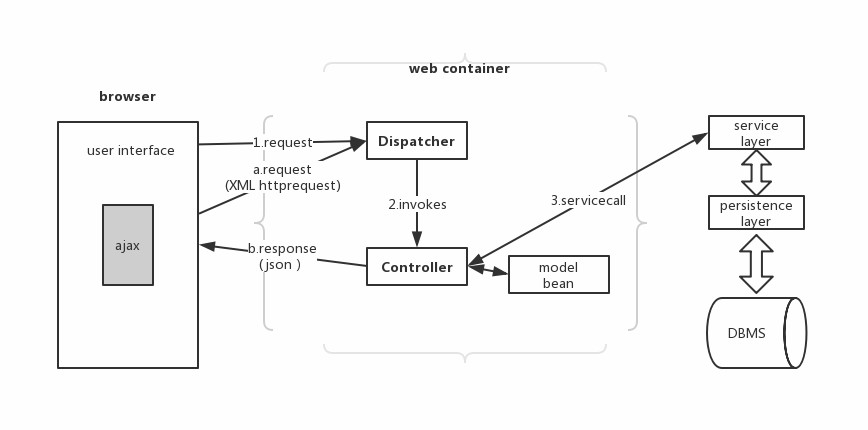
\includegraphics[width=1.0\linewidth]{figure/BS_structure}
	\caption{B/S架构图}
	\label{fig:BS_structure}
\end{figure}

\subsubsection{RESTful API}

REST全称是Representational State Transfer,中文意思是表述(编者注:通常译为表征)性状态转移。

RESTful API有以下的特征:

(1)每一个uri代表一种资源。

(2)客户端和服务器之间,传递这种资源的某种表现层。

(3)客户端通过四个HTTP动词(GET、POST、DELETE、PUT),对服务器端资源进行操作,实现"表现层状态转化"(增删改查)。

(4)URL中通常不出现动词,只有名词。

(5)使用JSON不使用XML。

\subsubsection{使用Redux存储网络请求状态}

Redux 是 JavaScript 状态容器,提供可预测化的状态管理。可以让你构建一致化的应用,运行于不同的环境(客户端、服务器、原生应用),并且易于测试。其使用Immutable数据结合React能让页面相应数据进行最小颗粒度的更新DOM结点。

\begin{figure}[thbp!]
	\centering
	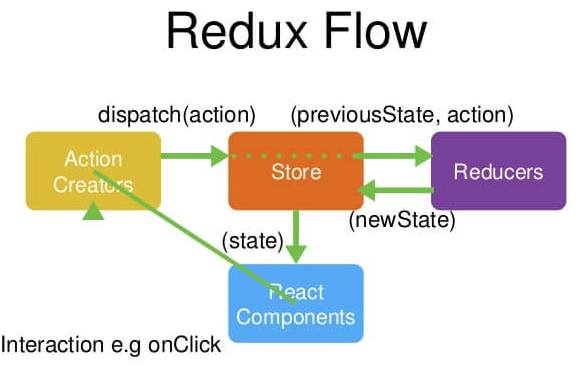
\includegraphics[width=1.0\linewidth]{figure/redux}
	\caption{redux数据流}
	\label{fig:redux}
\end{figure}

每一次发起http请求获得响应的时候触发一个Redux Action,将服务端返回的数据存储在store中。这样做的好处是所有的需要使用服务端数据的React组件不需要影响父子组件之间的数据流直接提取公用的状态。

\subsection{账号系统}

\subsubsection{密码加密}

\begin{lstlisting}[language=C]
@property
def password(self):
	raise TypeError("cannot read a user's password")

@password.setter
def password(self, password):
	self.password_hash = generate_password_hash(password)

def verify_password(self, password):
	if not password:
		return False
return check_password_hash(self.password_hash, password)
\end{lstlisting}

\begin{center}
	{\small 用户密码的创建和验证}
\end{center}

@property装饰器装饰一个属性的getter,修饰的函数名为属性名,返回的值是该属性的getter,此处该属性不能直接访问访问则会抛出异常。

@property同时会全局创建一个@password.setter的装饰器装饰属性的setter,在设置password的时候我们其实设置的是password\_hash这个属性,值为hash加密过的password。

处理登陆请求的时候调用verify\_password函数判断密码是否正确。

这样做的好处就是即使是数据库管理员也不可能知道用户的密码,只能看到加密后的字符串,同时md5是不可逆的加密方式,不能由加密后的字符串反推出明文,保证了数据的机密性。

\subsubsection{邮箱验证}

用户注册和忘记密码的时候需要使用邮箱验证。在用户注册成功后会创建一个用户独有的token,将token作为链接参数发送给用户邮箱中,在用户点击链接进入验证页面的时候会将token返回后端后端进行验证。

验证失败有两种结果,一是token过期,二是token中的用户信息不匹配当前用户。通常不匹配的情况有三种:

(1) 用户自己改了url中的token

(2) 中间商劫持被修改了token信息。

(3) 非法重定向。

无论哪种都是非法篡改token的行为,影响用户信息安全。

\begin{figure}[thbp!]
	\centering
	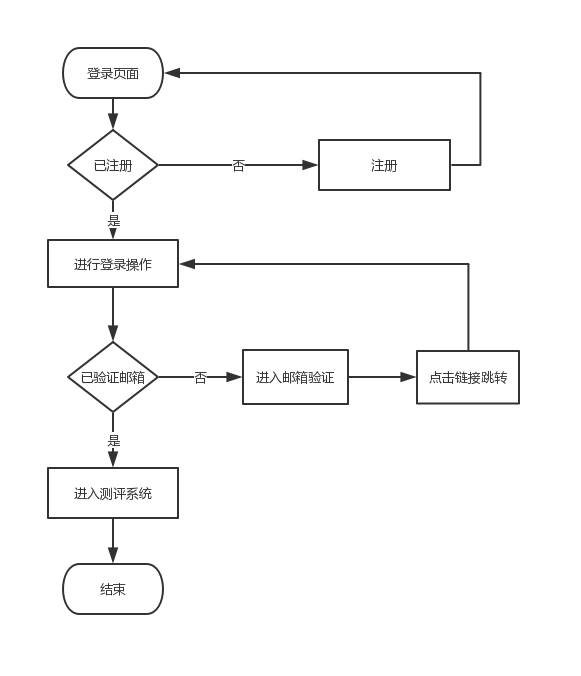
\includegraphics[width=1.0\linewidth]{figure/register_email}
	\caption{注册邮箱激活}
	\label{fig:register_email}
\end{figure}

\begin{figure}[thbp!]
	\centering
	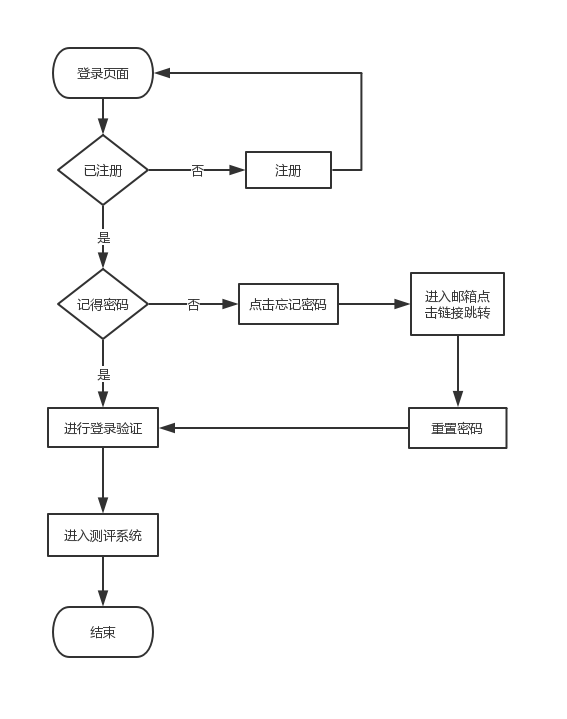
\includegraphics[width=1.0\linewidth]{figure/password_mail}
	\caption{忘记密码邮箱验证}
	\label{fig:password_email}
\end{figure}

\subsection{评测与数据分析}

\subsubsection{上传试卷}

\begin{figure}[thbp!]
	\centering
	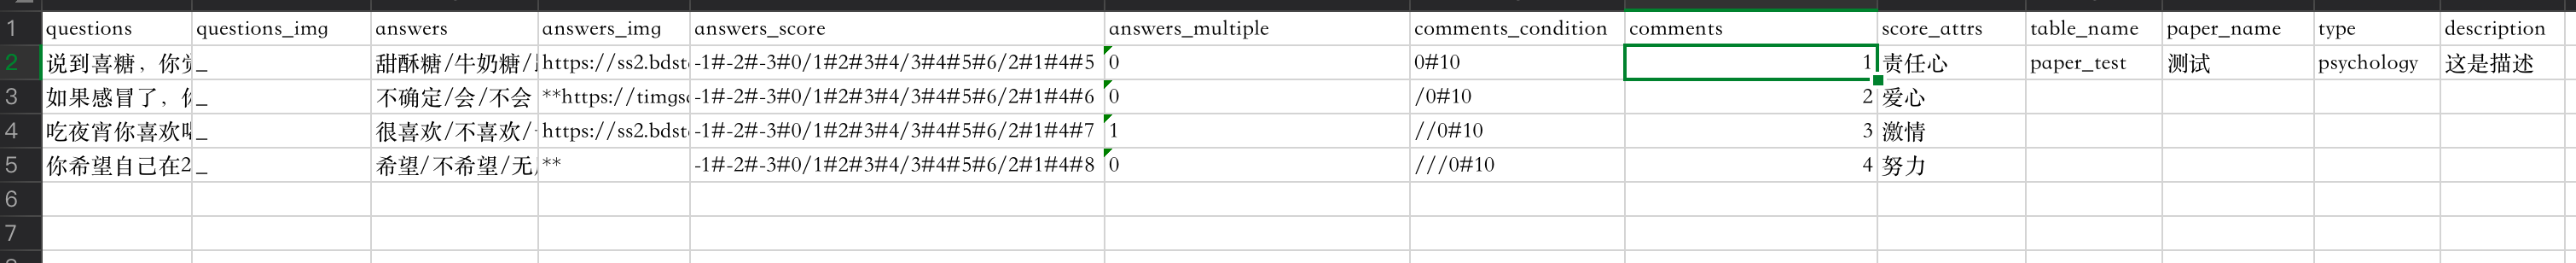
\includegraphics[width=1.0\linewidth]{figure/paper}
	\caption{示例试卷}
	\label{fig:paper}
\end{figure}

\begin{figure}[thbp!]
	\centering
	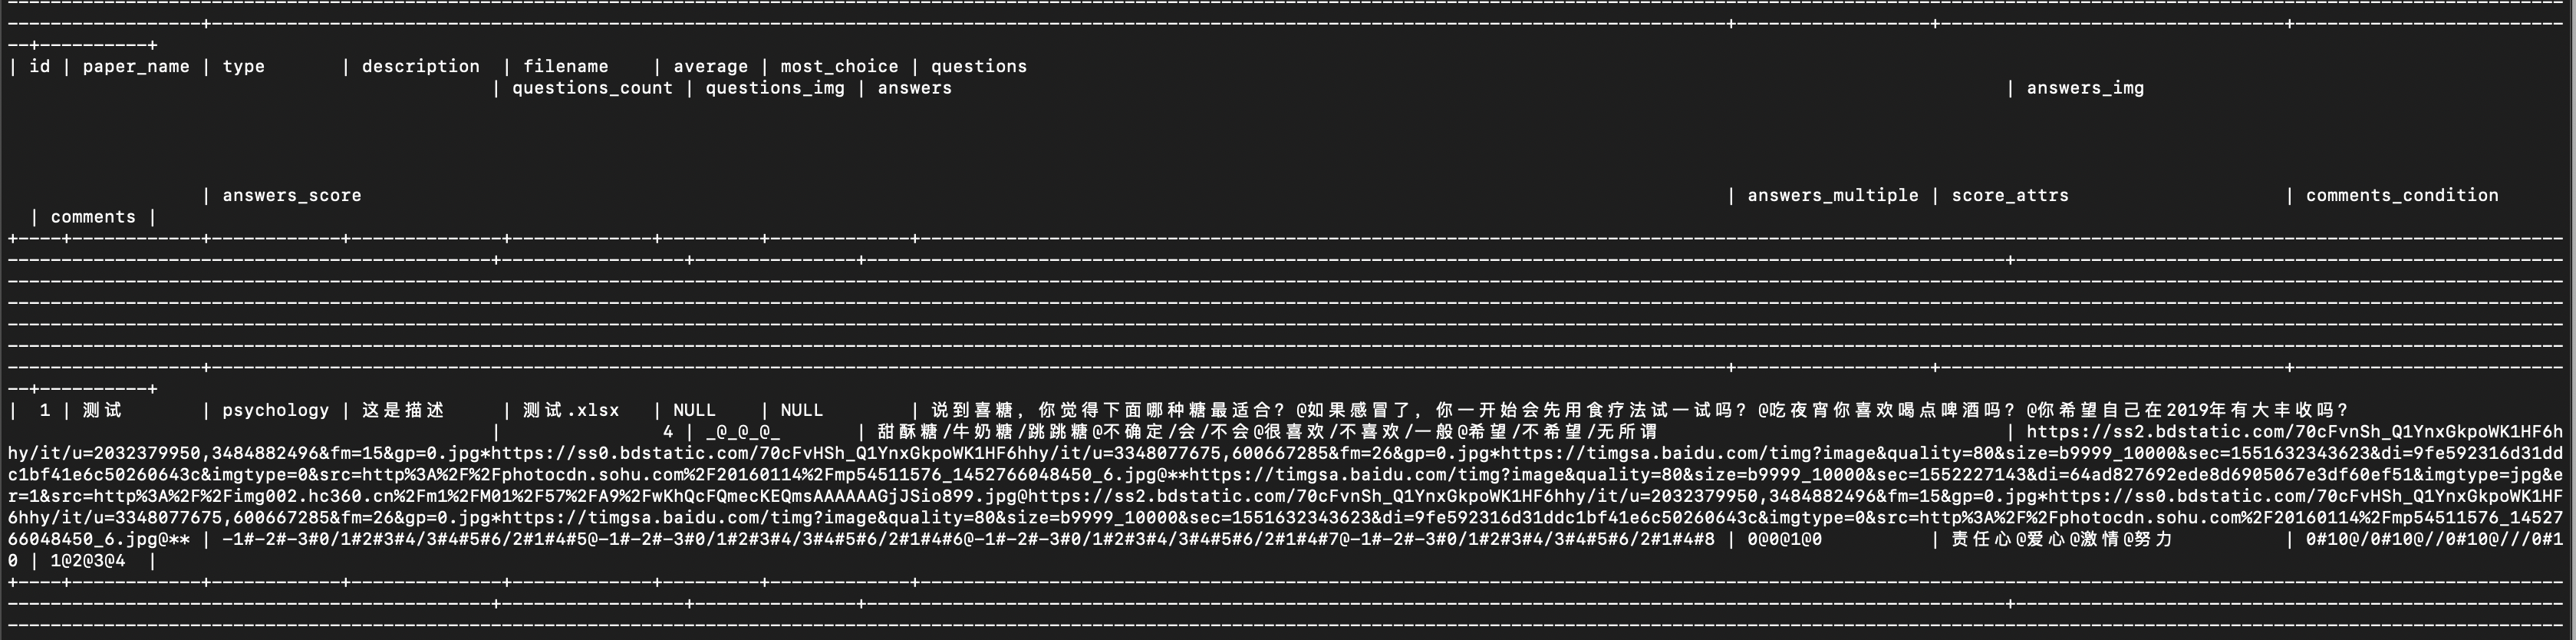
\includegraphics[width=1.0\linewidth]{figure/paper_database}
	\caption{试卷表}
	\label{fig:paper_database}
\end{figure}

上传试卷是通过上传excel表格。

questions 问题的题目

questions\_img 题目的配图的图片链接地址

answers 题目的答案,答案之间用"/"来进行分割

answers\_img 题目答案的配图的图片链接地址,配图之间用"*"进行分割,只支持一个答案只有一个配图

answers\_score 对应每个答案对应试卷指标的分数加成,正数为增加,负数为减少,0则表示该答案对此项指标没有影响,每个答案之间用"/"分隔,每个指标之间用"\#"分隔

answers\_multiple 该题目是否是多选,0表示单选,1表示多选

comments\_condition 试卷各种评论的条件,每个指标之间用"/"分隔,0\#10表示该指标大于零小于10

comments 具体的评论内容

score\_attrs 试卷的得分指标

table\_name 数据库中的表名

paper\_name 试卷名称

type 试卷的类型,psychology代表室心理评测,grade代表普通试卷,决定了试卷的算分机制

description 试卷的描述

上传文件后后端通过读取excel表格文件将数据插入到数据库中。

每个问题之间的数据使用"@"来进行连接。

在评测时候后端会对表数据进行解析和构建对象发送给前端。

\begin{figure}[thbp!]
	\centering
	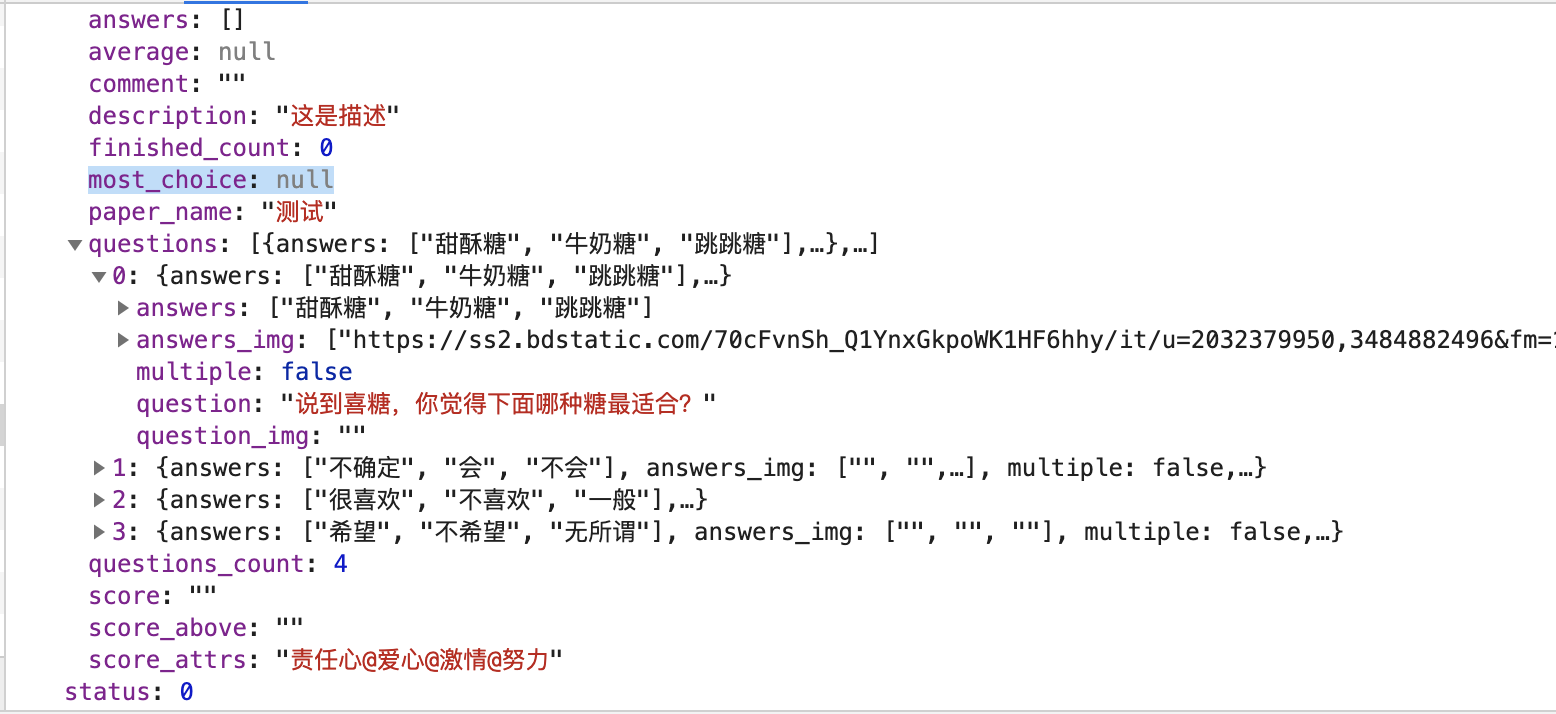
\includegraphics[width=1.0\linewidth]{figure/paper_data}
	\caption{试卷数据结构}
	\label{fig:paper_data}
\end{figure}

其中average、comment、most\_choices、answers、score、score\_above、score\_attrs是完成试卷以后才会有的参数,与数据分析结果的接口是一个接口。

\subsubsection{数据分析}

\begin{figure}[thbp!]
	\centering
	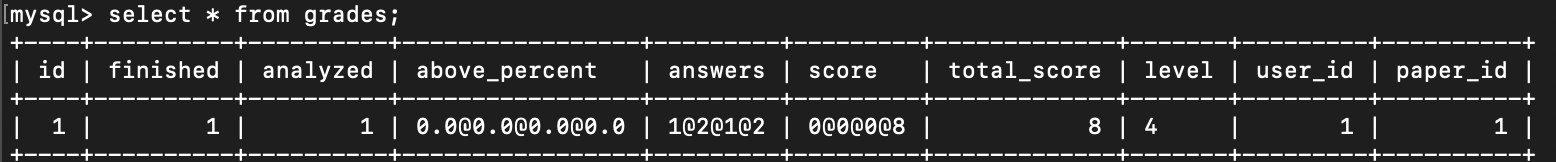
\includegraphics[width=1.0\linewidth]{figure/grade}
	\caption{成绩数据表}
	\label{fig:grade}
\end{figure}

用户回答完后,答案之间以"@"分隔开来进行存储。在计算得分的时候遍历答案进行指标的加减。

\subsubsection{计算每个问题最多回答的答案}

\begin{lstlisting}[language=C]
most_choice = "@".join(map(lambda x: Counter(x)
		.most_common(1)[0][0], choices))
\end{lstlisting}

Counter是Python内置的一个计数器类,可以得到每个元素出现的次数,其中.most\_common函数可以得到列表中出现频率最频繁的元素。
